\RequirePackage{amsthm} %https://tex.stackexchange.com/questions/687324/unknown-theoremstyle-warning-with-springer-nature-template
\documentclass[sn-mathphys-num,iicol]{sn-jnl}

%\usepackage{sn-jnl.sty}
\usepackage{graphicx}%
\usepackage{multirow}%
\usepackage{amsmath,amssymb,amsfonts}%
\usepackage{amsthm}%
\usepackage{physics}
\usepackage{siunitx}
\usepackage{mathrsfs}%
\usepackage[title]{appendix}%
\usepackage{xcolor}%
\usepackage{textcomp}%
\usepackage{manyfoot}%
\usepackage{booktabs}%
\usepackage{algorithm}%
\usepackage{algorithmicx}%
\usepackage{algpseudocode}%
\usepackage{listings}%
\usepackage{newtxmath}%
\usepackage[tiny]{titlesec}%
%\usepackage[ngerman]{babel}
\usepackage{enumitem}

\theoremstyle{thmstyleone}
\newtheorem{theorem}{Theorem}
\newtheorem{proposition}[theorem]{Proposition}

\theoremstyle{thmstyletwo}
\newtheorem{remark}{Remark}

\theoremstyle{thmstylethree}
\newtheorem{definition}{Definition}

\raggedbottom

\newcommand{\td}{\text{d}}

\titleformat{\subsection}{}{\thesubsection}{1em}{\itshape}
\titleformat{\subsubsection}{}{\thesubsubsection}{1em}{\itshape}

\begin{document}
        
\title[]{Particle Detectors and Instrumentations}
\author*[1]{\fnm{Jonas} \sur{Wortmann}}\email{s02jwort@uni-bonn.de}
\author*[1]{\fnm{Marc} \sur{Hauer}}\email{s65mhaue@uni-bonn.de}
\affil*[1]{Rheinische Friedrich--Wilhelms--Universität, Bonn}

\maketitle

\section{Introduction}

\section{Theory}

\section{Cosmic Data}
\subsection{Experimental Setup}
\subsection{Experimental Procedure}
% micromegas detector & szintillators & trigger logic & DAQ



\section{Multiple Scattering}
\subsection{Experimental Setup}
To observe multiple scattering, a electron beam of $\SI{2.9}{GeV}$ is provided by the stretcher ring of ELSA, whose exit is shown in \autoref{fig:beam_setup_elsa}. The setup of the micromegas detector with the scintillators and the trigger logic, used and tested with the cosmic data, is placed a few meters in front of the output of the accelerator, such that the beam hits the detector as seen in \autoref{fig:detector_setup_elsa}. This is ensured by a laser, build in at the end of the accelerator, which could be slid into the middle of the opening to point along the beam line. However, it is known that the laser points a few centimeters too low compared to the actual beam. This must be note by constructing the setup and while placing the targets.
To do latter, a metal bar is mounted close to the detector thus the targets could be placed in a distance between $\SI{5.5\pm 0.5}{cm}$ and $\SI{105.5\pm 0.5}{cm}$ to the first scintillator into the beam, where the uncertainties come from the measuring tape used to evaluate these distances. Thereby, the laser is used to adjust the bar and to ensure a free beam path up to the detector or the placed material.
The available materials with their thicknesses are listed in \autoref{tab:available_materials}. These were measured by a previous group with a caliper, so uncertainties of $\SI{0.1}{mm}$ are assumed, which is roughly checked with the maesuring tape.


\begin{table}\centering
  \renewcommand*{\arraystretch}{1.1}
  \begin{tabular}{c|c||c|c}
    \multicolumn{2}{c||}{Aluminum} & \multicolumn{2}{c}{Copper} \\
    {\fontsize{8}{3}\selectfont $d/\si{cm}$} & {\fontsize{8}{3}\selectfont \#} & {\fontsize{8}{3}\selectfont $d/\si{cm}$} & {\fontsize{8}{3}\selectfont \# } \\\hline \rule{0pt}{3ex}
    \num{1.22\pm 0.01} & 2 & \num{0.2\pm 0.01} & 3 \\
    \num{2.5\pm 0.01} & 1 & \num{0.5\pm 0.01} & 2 \\
    \num{5\pm 0.01} & 1 & \num{1.48\pm 0.01} & 2 \\
    \num{9.96\pm 0.01} & 1 & & \\
    \num{9.93\pm 0.01} & 1 & & \\
  \end{tabular}\vspace{3mm}
  \caption{Available scattering materials of thickness $d$ and quantity $\#$.}
  \label{tab:available_materials}
\end{table}

\begin{figure}
  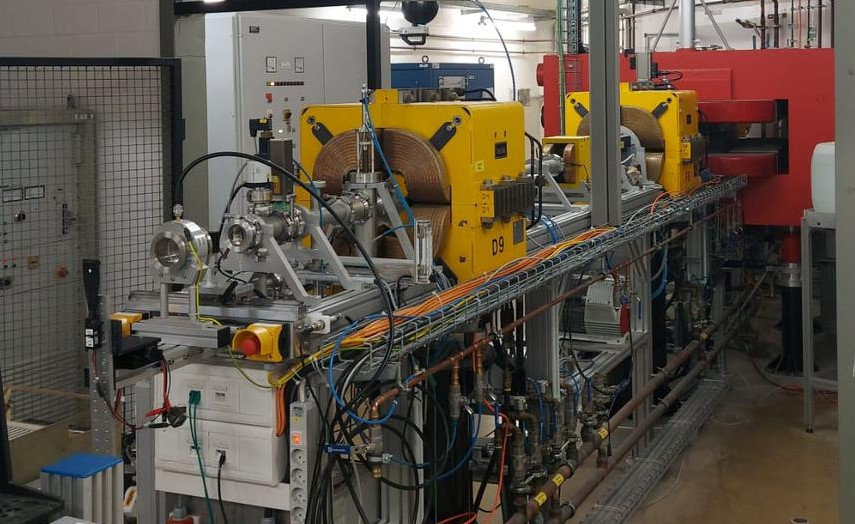
\includegraphics[width=\linewidth]{figures/beam_setup_elsa.jpg}
  \caption{Exit of ELSA.}
  \label{fig:beam_setup_elsa}
\end{figure}

\begin{figure}
  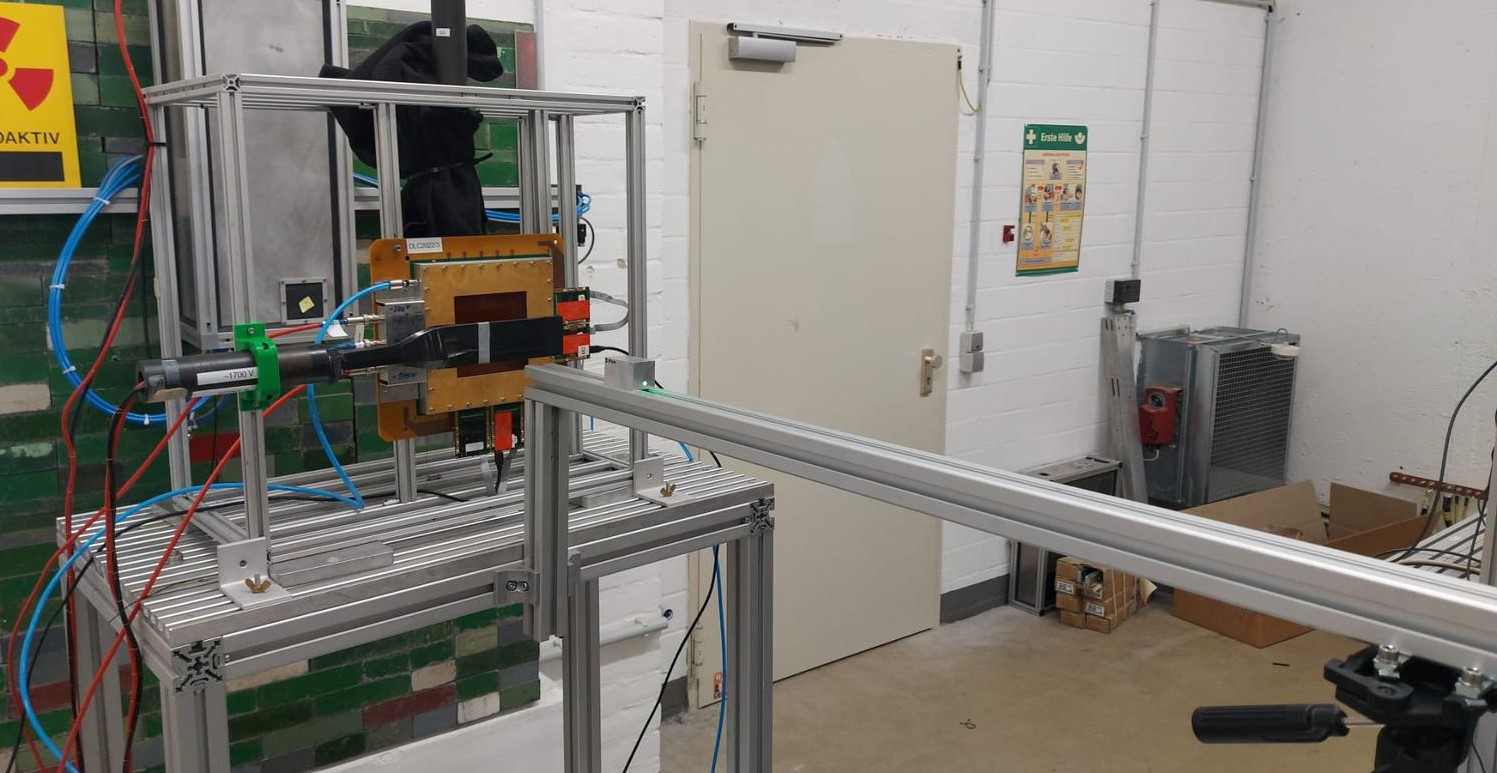
\includegraphics[width=\linewidth]{figures/detector_setup_elsa.jpg}
  \caption{Setup of the detector and the metal bar, to place the targets on it and align them with the green laser.}
  \label{fig:detector_setup_elsa}
\end{figure}

\subsection{Experimental Procedure}
After controlling the setup of the detector including the trigger logic and the right adjustment of the metal bar, a test run without any target in the beam is performed, to ensure the functionality of the setup and the data taking program DAQ.
Afterwards, for both materials multiple runs are recorded. Thereby the thicknesses $D$ of the targets are always chosen to be different multiples of the radiation length $X_0$ of the material, namely $0.5$, $1$ and $2$ times the length. The exact configurations for the different recordings are listed in \autoref{tab:config_materials}.
(...)

\begin{table}\centering
  \renewcommand*{\arraystretch}{1.15}
  \begin{tabular}{c|c|c}
    $D/X_0$ & Aluminum & Copper \\
    & {\fontsize{7}{5}\selectfont ($X_0=\SI{8.897}{cm}$)} & {\fontsize{7}{5}\selectfont ($X_0=\SI{1.436}{cm}$)} \\\hline\rule{0pt}{6ex}
    $0.5$ & \num{5} & $\begin{array}{r}
                \num{0.5} \\
                +\,\num{0.2} \\\hline
                =\,\num{0.7}    
              \end{array}$ \\\hline
    $1$ & \num{9.93} & \num{1.48} \\\hline
    $2$ & $\begin{array}{r}
      \num{1.22} \\
      +\,\num{2.5} \\
      +\,\num{5} \\
      +\,\num{9.93} \\\hline
      =\,\num{18.65}
    \end{array}$ & $\begin{array}{r}
                      2\times\num{1.48} \\\hline
                      =\,\num{2.96}
                    \end{array}$ \\\hline
    $3$ & $\begin{array}{r}
      \num{2.5} \\
      +\,\num{5} \\
      +\,\num{9.93} \\
      +\,\num{9.96} \\\hline
      =\,\num{27.39}
    \end{array}$ & $\begin{array}{r}
                      2\times\num{0.2} \\
                      +\,2\times\num{0.5} \\
                      +\,2\times\num{1.48} \\\hline
                      =\,\num{4.36}
                    \end{array}$ \\\hline
  \end{tabular}\vspace{3mm}
  \caption{Specific configurations of used materials with radiation length $X_0$ and overall thicknesses $D$.}
  \label{tab:config_materials}
% uncertainties and units
\end{table}





\clearpage
\section{Analysis ELSA (\textbf{temporary informations})}
Here is a quick rundown of how the analysis for ELSA works.

The way that the data taking works is that the detector triggers about every $\SI{25}{ns}$ and reads all strips.
It needs some time to reset and then does it again.
For ELSA data will be lost at downtime and the detector will basically trigger continuously because of the steady electron beam.

The data will be such that one event (i.e.\ one trigger) contains (most probably) multiple hits (i.e.\ multiple strips fire / register a hit).
Ideally, one would like only a single electron registered as a single hit.
This poses a problem because there are many different reasons for the undesired multiple hits.
\begin{enumerate}[label=\arabic*)]
  \item There is a certain noise on the detector, which will be registered as a hit, but this only deposits very little charge.
    To filter these events there is a certain charge threshold.
  \item It is possible, that a beam-electron creates a $\delta $-electron in the material and both hit the detector.
    This will be seen as two separate hits.
  \item The electron has a very high energy and as it traveles through the air, it is possible that it interacts with the air molecules.
    This interaction could be inelastic scattering, which would result in a Hadron shower (most likely pions) on the detector.
    This is seen (often) as a single hit (which is the electron; this hit can be very far from the expected distribution because it scattered under a higher angle) and a bunch of hits close together (Hadrons).
    To filter these events one can count the number of independent strip(s) that fired.
    Independes here means a strip or multiple strips next to each other give a signal and the adjacent strips to the left and right give none.
    These strips are called clusters.
    For example: \\\texttt{...|...||......||||..|.||.|..}\\
    would be 6 clusters.
    If the number of clusters in a single event is greater than a certain number $x$ (currently $x=2$), then this event will be left out.
\end{enumerate}
There will be a number of histograms, this includes: x and y strip events, clusters, cluster size, xy hitman etc.\

For the analysis a gaussian curve is fittet to the histogram: y strip events.
The x strips don't work well (probably detector issue and the beam has an elliptic profile).
The standard deviation of the curve is related to $\theta $ via $\tan \theta =\tfrac{\sigma }{d}$ with $d$ the distance between the target and the detector.
First calculations with this formula are in the right order of magnitude.
This will probably work better with a more precise filtering of the available data.

To evaluate the theory, $$\theta _\text{exp}=\arctan\left(\dfrac{\sigma }{d}\right)$$ is plotted against $$\theta _\text{theo}=\text{const}\,\sqrt[]{\dfrac{x}{x_0}}\left(1+0.038\ln\left(\dfrac{x}{x_0}\right)\right).$$
This should give a linear correlation between these two values thus verifying the proportionality i.e.\ the theory.
\textbf{Currently there is no correlation at all between these two so WIP.}

%\bibliography{refs}

\end{document}
